\pdfoutput=1
\documentclass[11pt]{article}

% Final version generation
% \usepackage[review]{acl}
\usepackage[]{acl}

\usepackage{graphicx}
\usepackage{caption}
\usepackage{subcaption}
\usepackage{tabularx}

% Standard package includes
\usepackage{times}
\usepackage{latexsym}
\usepackage{amsmath}
\usepackage[shortlabels]{enumitem}



% Latin characters
\usepackage[T1]{fontenc}

% UTF8 Encoding 
\usepackage[utf8]{inputenc}

% Space saver
\usepackage{microtype}

% Alias for pcr police
\newcommand{\pol}[1]{{\fontfamily{pcr}\selectfont#1}}

\usepackage{cuted}


\title{
BERT, RoBERTa and T5 transformers implementations \\ 
for Detection of Propaganda Techniques in News Articles.\\
\vspace{0.2cm}
\small Natural Language Processing Project Paper, Fall 2021
}

\author{
Antoine Basseto,
Giacomo Camposampiero 
\and Andrea Pinto \\         
ETH Zurich - Swiss Federal Institute of Technology \\ 
\texttt{\{abasseto, gcamposampie, pintoa\}@ethz.ch}
}

\begin{document}
\begin{strip}
    \centering
    \textbf{\Large BERT, RoBERTa and T5 transformers implementations \\ 
    for Detection of Propaganda Techniques in News Articles.}\\
    \vspace{0.2cm}
    \textbf{\large Intermediary Paper Report} \normalsize
    \vspace{4mm}
\end{strip}

\section*{Progress report notes}
Since the project proposal was submitted on November 1st, our team focused on designing an architecture that could handle \pol{RoBERTa} and \pol{T5} technologies for propaganda detection. We propose below a novel approach to solve both the span identification (\pol{SI}) and the technique classification (\pol{TC}) sub-tasks.

Although the result section is still mostly empty in this paper, we already have functional running models for both \pol{SI} and \pol{TC} tasks.
Our entire code work is visible on our public GitHub repository\footnote{ \url{https://github.com/andreakiro/nlpropaganda}}.

\subsection*{Reshaping the scope of the project}
Recall now that the objective we defined in our project proposal was two-fold:
\begin{enumerate}
    \item To implement different models able to automatically detect the use of propaganda techniques in text snippets, accomplishing both the \pol{SI} and \pol{TC} sub-tasks of the shared task.
    \item To compare the implemented models and draw conclusions on their performance through an error analysis for each of them.
\end{enumerate}
We proposed to fulfill Goal (1) with the following:
\begin{enumerate}[(a)]
    \item A small self-trained language model to provide a baseline performance we can compare other models to.
    \item \pol{RoBERTa} \cite{roberta}, a state-of-the-art pre-trained model based on the Transformer architecture.
    \item \pol{T5} \cite{2020t5}, another state-of-the-art Transformer based architecture that uses a text-to-text approach.
\end{enumerate}
So far, we have spent our time designing and implementing a modular architecture, which would allow us to smoothly integrate different models.
Because we are confident in our ability to further enhance our architecture, we have decided to focus on pre-trained language models (PLMs), and not to develop our own self-trained language model from scratch (as said in (a)). Therefore, we will use \pol{BERT} as our new baseline model, to compare the effects of different \pol{PLM}s.

\subsection*{Remaining objectives}
To conclude the project, we would like to:
\begin{enumerate}
    \item Solve the problems we're currently facing with our architecture. 
    \begin{enumerate}
        \item Fine tuning the weights for the \pol{SI} model, introduced to combat class imbalance, our model now predicts too many spans as being propaganda (this behaviour can be observed interpreting the results in Table \ref{table:si-results}).
        \item Memory management problems in PyTorch, that prevent us from successfully training our model using GPUs.
        \item Find correct weights for our \pol{TC} model to combat class imbalance.
    \end{enumerate}
    \item Fine-tune our architecture using different state-of-the-art \pol{PLM}s, changing hyperparameters and adding regularization methods.
    \item Train multiple epochs of our models on the Euler ETH cluster GPUs to better fit them.
    \item Implement a final predictions writer to create human readable output, allowing us to feed our model any kind of text to retrieve the fragments classified as propaganda from it, and the technique associated with each of them.
    \item Possibly exploring the implementation of add-on features to our architecture such as conditional random field (\pol{CRF}) or data augmentation techniques such as \textit{back translation}, \textit{random replacement} and \textit{random insertion} in order to further enhance the results.
    \item Compare the implemented final models and draw conclusions on their performance through a complete error analysis.
\end{enumerate}

\maketitle
\begin{abstract}
This paper describes the design of our system contributing to the Task 11 of SemEval-2020 \cite{semeval} aiming to detect propaganda techniques in news articles.
We investigate a novel approach allowing the technique classification task (\pol{TC}) to work under relaxed assumptions and be more easily applicable to real-world scenarios, leading to changes in the span identification task (\pol{SI}) as well.
% We investigate a novel architecture using the span identification task (\pol{SI}) as a preprocessing stage of the technique classification task (\pol{TC}), performing an additional pruning and focusing our technique classification only on spans that may already contain a propagandist argument.
Both models are built on top of heterogeneous pre-trained language models (\pol{PLMs}) such as \pol{BERT}, \pol{RoBERTa} and \pol{T5}.
The described architecture achieved an F$_1$-score of $0.29651$ on the \pol{SI} task (ranking $34/45$) and an F$_1$-score of $X$ on the \pol{TC} task (ranking $X/45$).
\end{abstract}

\section{Introduction}
The proliferation of online misinformation has led to a significant amount of research into the automatic detection of fake news \cite{fakenews}. However, most of the efforts have been concentrated on whole-document classification \cite{rashkin-etal-2017-truth} or analysis of the general patterns of online propaganda \cite{garimella2015, chatfield2015}, while little has been done so far in terms of fine-grained text analysis. This approach could complement existing techniques and allow the user to extract more informed and nuanced judgment on the piece being read. Moreover, it could also inform journalists on the pitfalls they might be falling into when writing articles.

In this context, Task 11 of SemEval-2020\footnote{The official task webpage: \url{https://propaganda.qcri.org/semeval2020-task11/}} \cite{semeval} aims to bridge this gap, facilitating the development of models capable of spotting text fragments where a defined set of propaganda techniques are being used. This shared task provides a well-annotated dataset of 536 news articles, which enables the participant to develop detection models that automatically spot a defined range of 14 propaganda techniques in written texts.

The focus of the task is broken down into two well-defined sub-tasks, namely (1) \textit{Span identification} \pol{(SI)} to detect the text fragments representative of a propaganda technique in the news articles and (2) \textit{Technique classification} \pol{(TC)} to detect the propaganda technique used in a given text span.

\section{Related Work}
\subsection{Literature review}
Literature regarding fine-grained propaganda detection and analysis has known a significant development only in the last few years, mostly thanks to the different shared tasks that covered this particular topic \cite{da-san-martino-etal-2019-findings, finalsemeval}.

One of the first contributions can be traced back to \cite{da-san-martino-etal-2019-fine}, which proposed a \pol{BERT}-based model to detect propaganda spans and to classify their techniques.
In the NLP4IF-2019 shared task, the participants used pre-trained language models (\pol{PLM}s), LSTMs and ensembles to tackle the problem of fine-grained propaganda classification \cite{yoosuf-yang-2019-fine, vlad-etal-2019-sentence, tayyar-madabushi-etal-2019-cost}.
Also in SemEval-2020 most of the winning teams solutions relied on Transformers and ensembles \cite{aschern, morio-etal-2020-hitachi-semeval, dimov2020nopropaganda, jurkiewicz2020applicaai}.

Our work is especially related to the cited studies of winning teams of the SemEval-2020 shared-task. We decided to use the same \pol{PLM}s as the other teams, with the addition of \pol{T5}, proposed by \cite{aschern} as an avenue of future work. However, we differ by tackling the \pol{TC} sub-task in a way none of the previous teams had explored, leading to other subtleties in the \pol{SI} sub-task as well.
% Our work is especially related to the cited studies of winning teams of the SemEval-2020 shared-task. We decided to use the same \pol{PLM}s as the other teams, with the addition of \pol{T5}, proposed by \cite{aschern} as an avenue of future work. However, we differ by tackling the \pol{SI} sub-task in a way none of the previous teams had explored, including other subtleties in the \pol{TC} sub-task as well.

\subsection{Pre-Trained Language Models (\pol{PLMs})}
In this study, three different types of Transformer-based \pol{PLM}s \cite{vaswani2017attention} were used to tackle the tasks (see Section \ref{sec:results}). \\
\textbf{\pol{BERT}} \cite{devlin2019bert} is the epoch-making Transformer-based masked language model. In our work, the \pol{BERT\textsubscript{LARGE}} model was employed. \\
\textbf{\pol{RoBERTa}} \cite{roberta} is a fine-tuned \pol{BERT}-based model where the authors investigated hyperparameters and training data size. \pol{RoBERTa} has achieved state-of-the-art results. In our work, the \pol{RoBERTa\textsubscript{LARGE}} model was employed. \\
\textbf{\pol{T5}} \cite{2020t5} is a state-of-the-art Transformer that uses a unified text-to-text approach. Encoder and decoder are similar in size and configuration to a \pol{BERT} stack. In our work, the \pol{T5\textsubscript{LARGE}} model was employed.

\subsection{Technology stack}
We opted to implement our architecture in \pol{AllenNLP} \cite{allennlp}, a recent NLP research library developed by the Allen Institute for Artificial Intelligence, built on top of PyTorch \cite{NEURIPS2019_9015} and SpaCy \cite{spacy2}, for developing state-of-the-art deep learning models on a wide variety of NLP tasks. 

% Kept here, maybe for the final draft
% \section{Glossary}
% - May be useful to briefly define once and for all the common concept and terms we are using and we'll use throughout the paper.

\section{Dataset}
\subsection{Data description}
The dataset used for the task, PTC-SemEval20 corpus \cite{semeval}, consists of a sample of news articles collected from mid-2017 to early 2019. The articles were retrieved from 13 propaganda and 36 non-propaganda news outlets, as labeled by Media Bias/Fact Check\footnote{https://mediabiasfactcheck.com}, and manually annotated by the organizers. The exact procedure of text labeling is discussed in depth in both \cite{da-san-martino-etal-2019-fine} and \cite{semeval}. 

The training and validation part of the corpus are the same as those presented in \cite{da-san-martino-etal-2019-fine}. The test part of the corpus consists of 90 additional news article in respect to the original evaluation articles, retrieved and annotated using the same procedure as the original. In total, the collection consists of 536 news articles containing 8,981 propaganda spans, that belong to one of the fourteen possible techniques.

\subsection{Data exploration}
Some statistics about the corpus (e.g. the number of instances and the average length in terms of tokens/characters for each propaganda technique, the average length of articles and others) were already given by the organizers as part of the shared task description paper \cite{semeval}.

In addition to this data, a more fine-grained exploration of the training corpus was performed as one of the first steps in the task tackling. The main reasons for this additional exploration were:
\begin{itemize}
    \item To extract meaningful insights that could be used to infer robust and effective heuristics for span pruning in \pol{SI} preprocessing, as discussed in Section \ref{sec:si:preprocesing}.
    \item To justify some of our model architecture choices, especially for the \pol{SI} model and its specificities we discuss in Section \ref{sec:si}.
\end{itemize}

Some of the results of this analysis have been reported in Figures \ref{fig:nb-sentences} and \ref{fig:nb-tokens}. Due to space constraints, other results (e-g. the distribution over token categories in gold spans and border tokens\footnote{Tokens near the beginning and end of a span.}), were omitted but can be accessed on our GitHub repository.

% \begin{figure}[h]
% \begin{subfigure}[b]{0.23\textwidth}
%   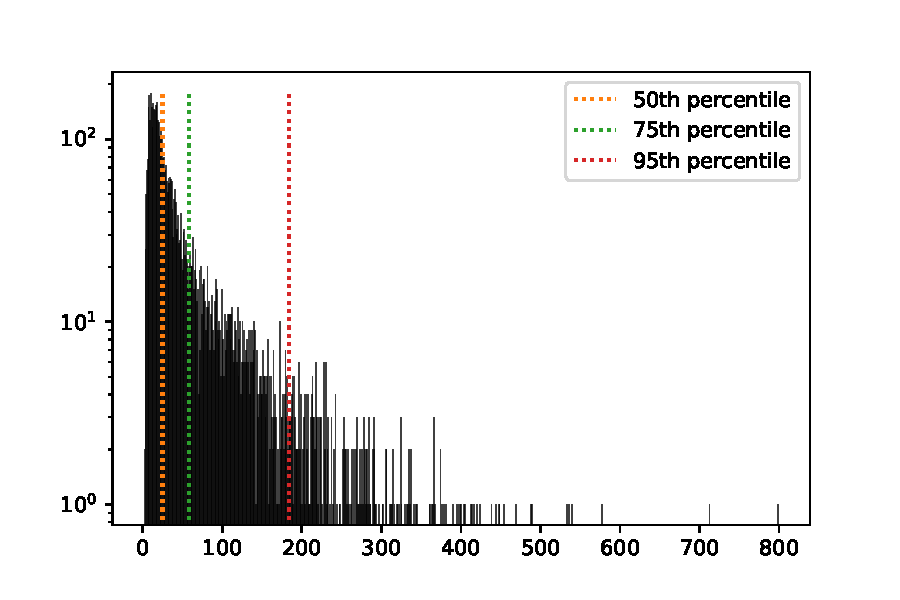
\includegraphics[width=\textwidth]{images/char_dist.pdf}
%      \centering
%   \caption{Character distribution in training gold spans.}
%   \label{fig:sfig1}
% \end{subfigure}
% \hfill
% \begin{subfigure}[b]{0.23\textwidth}
%   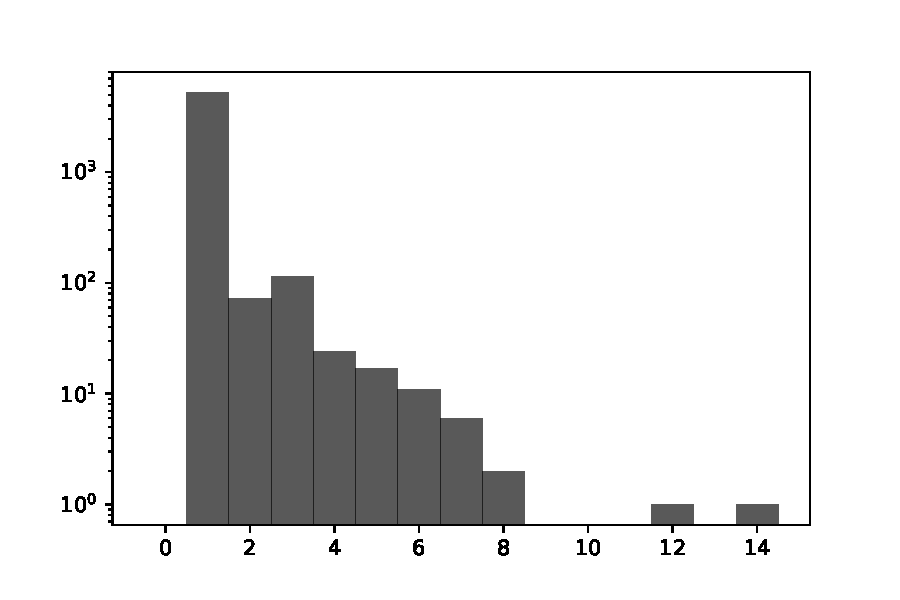
\includegraphics[width=\textwidth]{images/sentences.pdf}
%   \caption{Number of sentences in training gold spans.}
%   \label{fig:sfig2}
% \end{subfigure}
% \hfill
% \begin{subfigure}[b]{.45\textwidth}
%     \centering
%   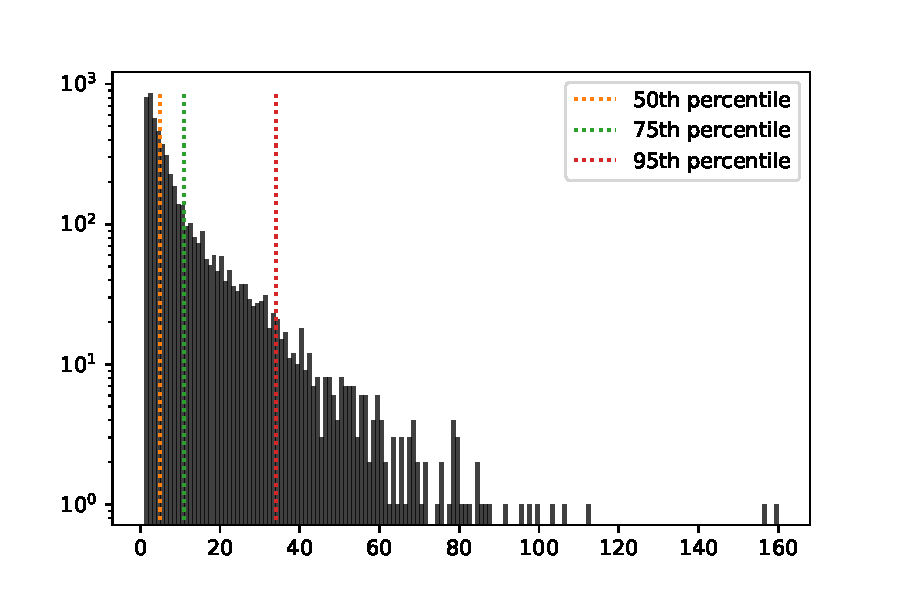
\includegraphics[width=.5\textwidth]{images/tok_dist.pdf}
%   \caption{Number of tokens in training gold spans.}
%   \label{fig:sfig3}
% \end{subfigure}
% \caption{Results of the data exploration of the training corpus.}
% \label{fig:exploration}
% \end{figure}

\begin{figure}[h]
    \centering
    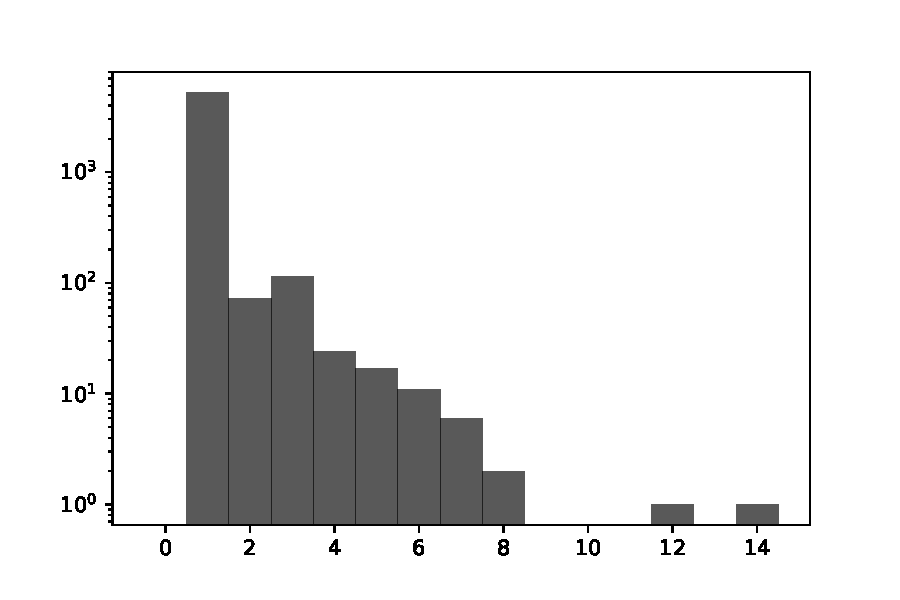
\includegraphics[width=0.4\textwidth]{images/sentences.pdf}
    \caption{Number of sentences in training gold spans.}
    \label{fig:nb-sentences}
\end{figure}
\begin{figure}[h]
    \centering
    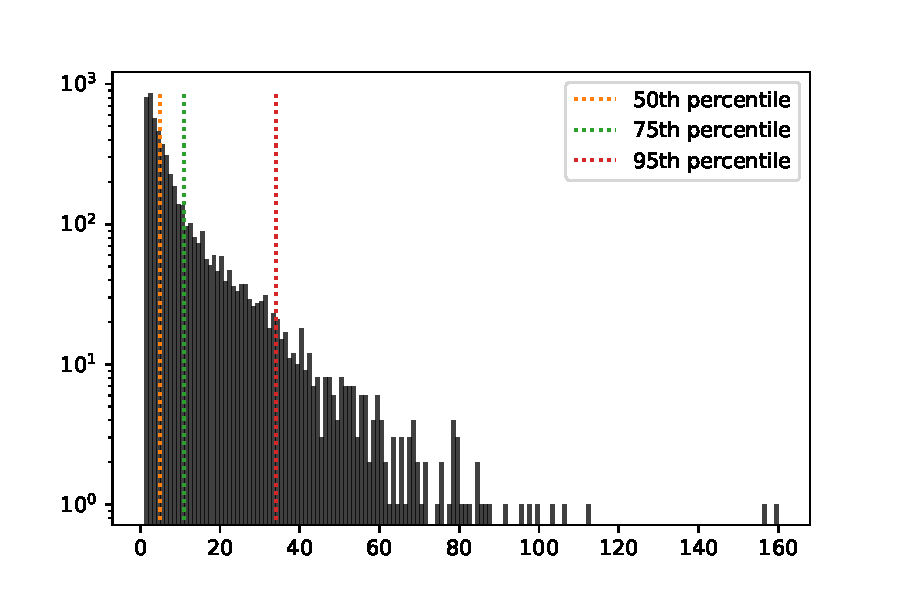
\includegraphics[width=0.4\textwidth]{images/tok_dist.pdf}
    \caption{Number of tokens in training gold spans.}
    \label{fig:nb-tokens}
\end{figure}

\section{System description} \label{sec:sys-desc}
Our approach was motivated by considering a real-world use of the \pol{TC} model. As described in the SemEval-2020 task, \pol{TC} models are supposed to classify a span as one of fourteen possible propaganda techniques, but this assumes that \pol{TC} models are always fed with spans that necessarily contain a propagandist argument. However, in a real-world scenario no such guarantees could be made, unless using a well-chosen list of manually selected spans.

\subsubsection*{Novel approach to architecture}
This conclusion resulted in two major changes compared to the architecture proposed in the SemEval-2020 shared task, leading to an approach where the \pol{SI} model is part of the preprocessing stage of \pol{TC}:
\begin{enumerate}
    \item \pol{TC} model should train on the results provided by the \pol{SI} model, and not on a given set of gold spans already known to be propaganda.
    \item Because the \pol{SI} model will make mistakes, the \pol{TC} model should also be able to handle false positives and predict spans as "\textit{Not Propaganda}", adding an extra 15th class.
\end{enumerate}

To provide additional means of fine-tuning the final architecture, we also decided to consider the \pol{SI} model as a span classification task rather than a sequence labeling task (see Section \ref{sec:si}). This meant that for each possible span, the \pol{SI} model assigns a probability of being a propagandist argument, and therefore lets the \pol{TC} model only classify spans that have this propaganda likelihood exceeding a well-chosen threshold. 
This way, we can regulate the number of false positives we forward on to \pol{TC} and make full use of the slackness offered by the added "\textit{Not Propaganda}" class. 

In this architecture, it could be argued that the addition of this new 15th label renders the \pol{SI} model unnecessary, but its use has strong computational advantages in allowing us to counteract the very heavy class imbalance we would have if we were considering every possible spans in the \pol{TC} task.

\subsection{Span Identification (\pol{SI})} \label{sec:si}
Span identification is often seen as a sequence labeling task, using Begin (\pol{B}), In (\pol{I}) and Out (\pol{O}) labels to classify each token as being in, out, or the beginning of a span. Despite the fact that many teams have used this common technique to model the problem, we decided to go another route and see it as a \textit{span classification} task. This means that we enumerate all possible spans in the article, filtering them with heuristics (see Section \ref{sec:si:preprocesing}), and we classify each of those as being a propaganda span or not. Our reasons for approaching this problem that way are the following:
\begin{itemize}
    \item To be able to use our \pol{SI} model as intended in our general pipeline (see Section \ref{sec:sys-desc}), we need a model that takes a span as input and classifies it as being propaganda or not, whereas a \pol{BIO}-tagging scheme would take a text as input and output the predicted propaganda spans.
    \item Furthermore, as seen in Figure \ref{fig:nb-sentences}, a non-negligible number of gold spans span multiple sentences. In some implementations from other teams, such as \cite{dimov2020nopropaganda}, using the \pol{BIO}-tagging scheme meant they were training a model that worked on each sentence individually, and they had to split gold spans spanning multiple sentences, negatively impacting their model's performance.
\end{itemize}


\subsubsection{\pol{SI} Preprocessing}  \label{sec:si:preprocesing}
To deal with the exponential number of spans in an article, we used heuristics to filter-out as many of them as possible. First of all, we only consider spans of 20 tokens or less. According to Figure \ref{fig:nb-tokens}, that means we can cover about 80\% of the gold spans in our training dataset. Second of all, we discard spans that consist exclusively of a combination of determinants, punctuation, space or \pol{EOL} tokens, as we can safely assume those will not be propaganda.


\subsubsection{\pol{SI} Embeddings} \label{sec:si:embedding}
After being extracted, spans are embedded. This is done by contextualising the text using a \pol{PLM}, and using that to have a contextualized representation of our span. The contextualized representation of our span is the result of concatenating the embedding of the first token of the span, the last token of the span, and an average of the token embeddings in the span weighted by a normalized self-attention score. That last part is the result of a self attentive span extractor module from \pol{AllenNLP}. Our results using different \pol{PLM}s can be seen in Section \ref{sec:results}. 

\subsubsection{\pol{SI} Loss function}
We are using the binary cross-entropy (BCE) loss to train our model. The use of the BCE loss is standard in binary classification tasks, but especially relevant in our case. Indeed, since the outputs of the \pol{SI} model will be used to prune spans given to the \pol{TC} model, we are not only interested in the classification but in the actual confidence our model has in it, because we can change the confidence threshold for which we discard spans or not in \pol{TC}. 

A specificity of our approach is also that it is affected by an important imbalance between the two classes. Only a small fraction of the spans that are retrieved by the preprocessing stage effectively contain a propagandist argument. To deal with this problem and prevent the model from classifying every span as not propaganda, we introduce a weight for the positive class in the loss function, defined as follows:
\begin{align*}
    weight_{+} = \frac{\#\ spans\ to\ classify}{\#\ propaganda\ spans}
\end{align*}
% where $s$ is to the number of spans that has to be classified and $g$ is the number of gold spans classified as propaganda.

\subsection{Technique Classification (\pol{TC})} \label{sec:tc}
The \pol{TC} model has to label each element of a set $S$ of spans with one of the 14 existing propaganda techniques. Note that this relies on the important assumption that the model is only provided with a set $S$ of spans which contain a propagandist argument. Recall also that our overall architecture is designed to consider the real-world scenario where this assumption cannot be made (see Section \ref{sec:sys-desc}). Our \pol{TC} model was intended to be built on top of the results of the \pol{SI} model. Consequently, we never have access to the ideal set $S$ but rather a relaxed set $S'$ of spans with the easier-to-satisfy assumption that $S \subset S'$. In order to correctly classify spans, we therefore had to add an extra label "\textit{Not Propaganda}" for spans containing no propagandist argument (i.e. belonging to $S'\backslash S$).

\subsubsection{\pol{TC} Preprocessing}
The key insight is that we can now think of the \pol{SI} model as applying \textit{an additional pruning} procedure on the set of possible spans.

For each article, we first apply the same preprocessing as we did for the \pol{SI} model. Namely, we enumerate all spans following the same heuristics described in Section \ref{sec:si:preprocesing}. We then use a pre-trained \pol{SI} model to get for each of those spans the probability of it containing a propagandist argument, and prune again according to those and a chosen threshold.

\subsubsection{\pol{TC} Embedddings}
After being extracted and pruned according to the results provided by the pre-trained \pol{SI} model, spans are embedded using the same techniques we employed for the \pol{SI} span embedding stage (see Section \ref{sec:si:embedding}). Our results using different \pol{PLMs} can be seen in Section \ref{sec:results}.

\subsubsection{\pol{TC} Loss function and metric}
We are using the standard cross-entropy (CE) loss to train our model. As in the \pol{SI} analog, this loss may suffer because of the design of our overall architecture. Indeed, depending on the threshold we set as a hyperparameter to filter the spans according to the results of the \pol{SI} model in the \pol{TC} preprocessing, we still could have much more false positives than real propaganda spans. This could lead to an important class imbalance and skew our model's predictions. To deal with this problem and prevent the model from classifying each of the new spans with the 15th label "\textit{Not Propaganda}", we introduce weights for each of the classes in the loss function, defined as follows {\textbf{\textit{(see point 1.(c) of Remaining objectives)}}}.

\begin{table*}[t]
\centering
  \begin{tabular}{|c|c c c|}
    \hline
    \textbf{Model} & \textbf{Custom F\textsubscript{1}} & \textbf{Precision} & \textbf{Recall} \\
    \hline
    \pol{\textbf{BERT}} & & & \\
    \pol{\textbf{RoBERTa}} & & & \\ 
    \pol{\textbf{T5}} & & & \\
    \hline
    \textbf{\pol{BERT}\textsubscript{\textit{test}}}  & 0.29651 & 0.17528 & 0.96147\\
    \hline
  \end{tabular}
  \caption{Model results on \pol{SI} task for validation and test data.}
    \label{table:si-results}
\end{table*}

\section{Experiments}
\subsection{Experimental setup}
The metric used to evaluate our \pol{SI} model is a custom F$_1$-measure that allows non-zero scores for partial matches between predicted and gold spans, as proposed in \cite{semeval}. 

The metric used to evaluate the \pol{TC} model is a standard micro-averaged F$_1$-measure.

\subsection{Experimental results} \label{sec:results}
Partial results obtained so far are included in Table \ref{table:si-results}.

\subsection{Error analysis}
A specific error analysis for both \pol{SI} and \pol{TC} will be included in the final paper. 
\begin{itemize}
    \item Analysis of portions of entirely missed, partially missed and entirely classified spans for each propaganda technique.
    \item Analysis of partially identified spans in \pol{SI}, to identify possible areas of improvements with post-processing.
    \item Visualization of a confusion matrix for classes in the \pol{TC} task, to have a simple representation of the which categories of propaganda are harder to classify for the model.
\end{itemize}

\section{Conclusion}
So far, results could be improved, but considering the initial stage of fine-tuning we are in, our approach seems to be of interest because of the advantages discussed throughout this paper.

\subsection{Future Work}
Because of the context of this project, and the time limit associated with it, we were not able to implement all of the ideas we had to improve our model. To build upon our work, we propose to look into the following:
\begin{itemize}
    \item Our architecture could be slightly modified, to give as an extra argument for the \pol{TC} model the confidence of the \pol{SI} model for its predictions in the form of the probability for each span. We expect this to be an important feature in determining whether a span belongs to the "\textit{Not Propaganda}" class or not for the \pol{TC} model.
\end{itemize}

% To add references without citing in text
\nocite{}

% Entries custom bib
\bibliography{custom}
\bibliographystyle{acl_natbib}

% \appendix
% \section{Example Appendix}
% \label{sec:appendix}
% In case we need an appendix.

\end{document}